\subsection{Deltaspike}

\begin{frame}[fragile]{Deltaspike}


\begin{itemize}
\item Framework che estende le funzionalità di CDI
\vspace{0.8em}
\item \textsl{Annotation-based}

\begin{lstlisting}[basicstyle={\tiny\ttfamily}]
&&@Secures&&
&&@AlterCompaniesAllowed&&
public boolean canUserAlterCompanies() {...}
\end{lstlisting}

\item Gestisce i permessi degli utenti
\end{itemize}


\end{frame}

\begin{frame}[fragile]{Architettura}
\begin{columns}[T]
\begin{column}{.5\textwidth}


\begin{itemize}
\item Sicurezza su base metodo

	\begin{itemize}
	\item Classe \textsl{Authorizer}
	\vspace{0.8em}
	\item Annotare i metodi\newline
	da controllare
	\end{itemize}

\vspace{0.8em}
\item Sicurezza su base pagina
	\begin{itemize}
	\item Gerarchia interfacce/classi -\textgreater  cartelle/pagine
	\vspace{0.8em}
	\item Interfaccia \textsl{AccessDecisionVoter}
	\vspace{0.8em}
	\item Possibilità di specificare\newline
	una pagina di errore\newline
	con un messaggio adatto
	\end{itemize}
\end{itemize}
\end{column}

\begin{column}{.5\textwidth}
\vspace{2.6em}
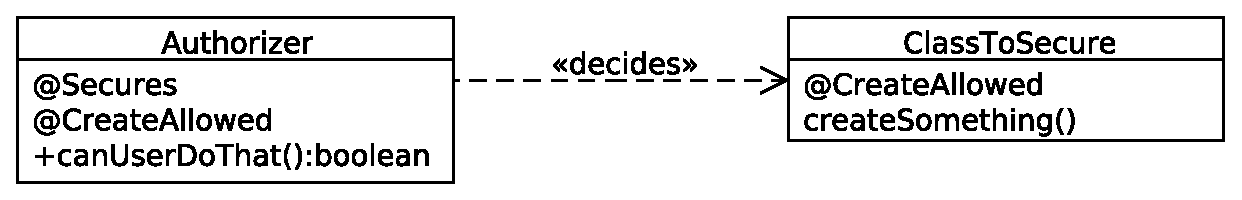
\includegraphics[width=1\textwidth]{deltaspikeMethod.eps}

\vspace{1.6em}
\begin{lstlisting}[basicstyle={\tiny\ttfamily}]

interface Pages{
    &&@Secured&&(value = { MyVoter.class }, 
    errorView = MyErrorPage.class)
    class AgreementWiz implements ViewConfig {
    }

    &&@Secured&&(value = { MyOtherVoter.class },
    errorView = MyOtherErrorPage.class)
    class Home implements ViewConfig {
    }
    
    class MyErrorPage {}
    class MyOtherErrorPage{}
}
\end{lstlisting}

\end{column}

\end{columns}
\end{frame}

\begin{frame}{Pagina di errore}
\centering
	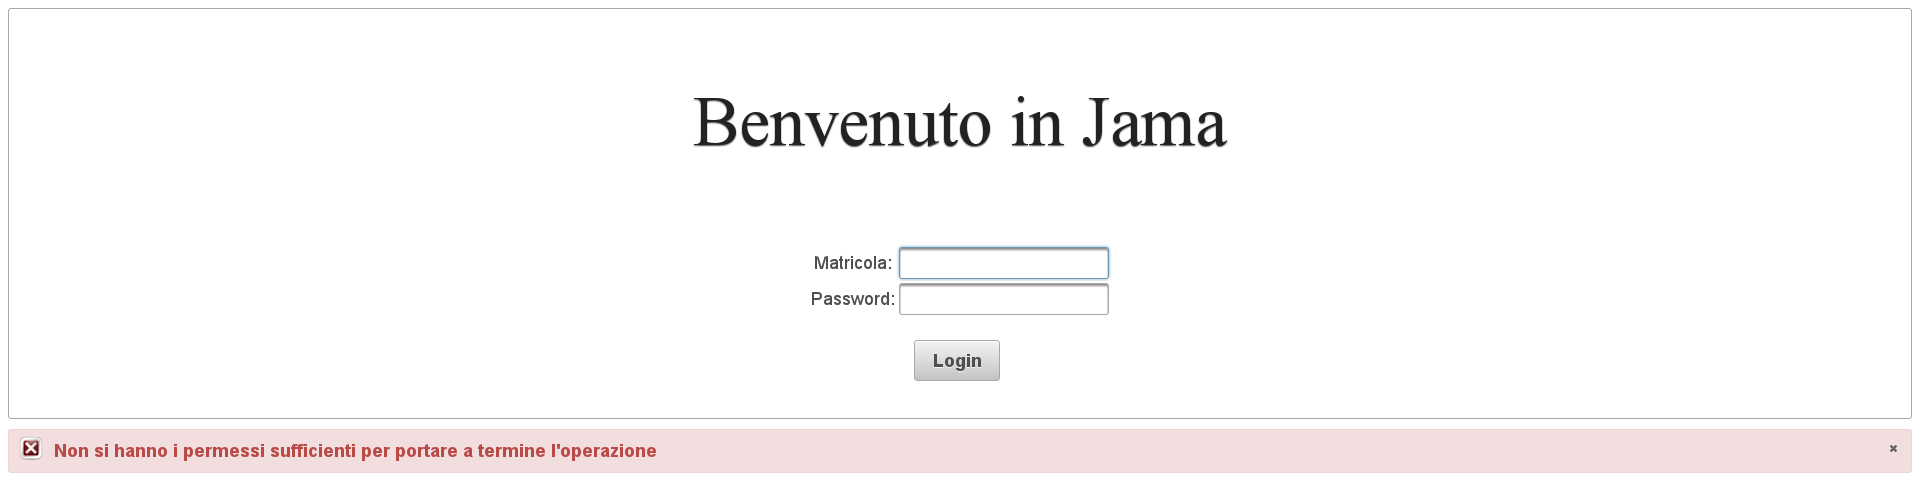
\includegraphics[width=1\textwidth]{PermessiInsufficienti.png}
\end{frame}

\subsection{LDAP}
\begin{frame}{Lightweight Directory Access Protocol}
\begin{columns}[T]
\begin{column}{.5\textwidth}
\begin{itemize}
\item Protocollo per accesso a cartelle
\item Utilizzato da Jama per recupero utenti
\item Libreria JLDAP
\end{itemize}
\end{column}

\begin{column}{.5\textwidth}
\vspace{0.7em}
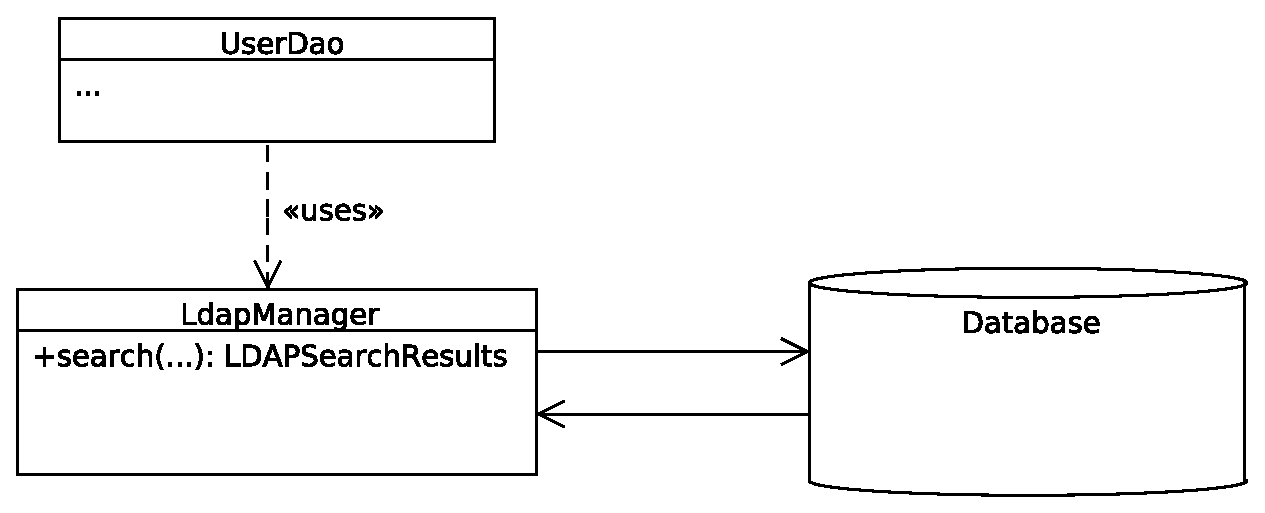
\includegraphics[width=1\textwidth]{Ldap.eps}
\end{column}




\end{columns}

\end{frame}


\section{Utenti}
\subsection{Modello}
\begin{frame}{Modello degli Utenti}
\begin{itemize}
\item Descrive la struttura delle classi riguardanti gli utenti\newline
ed i loro permessi
\end{itemize}	

\vspace{0.8em}
\centering
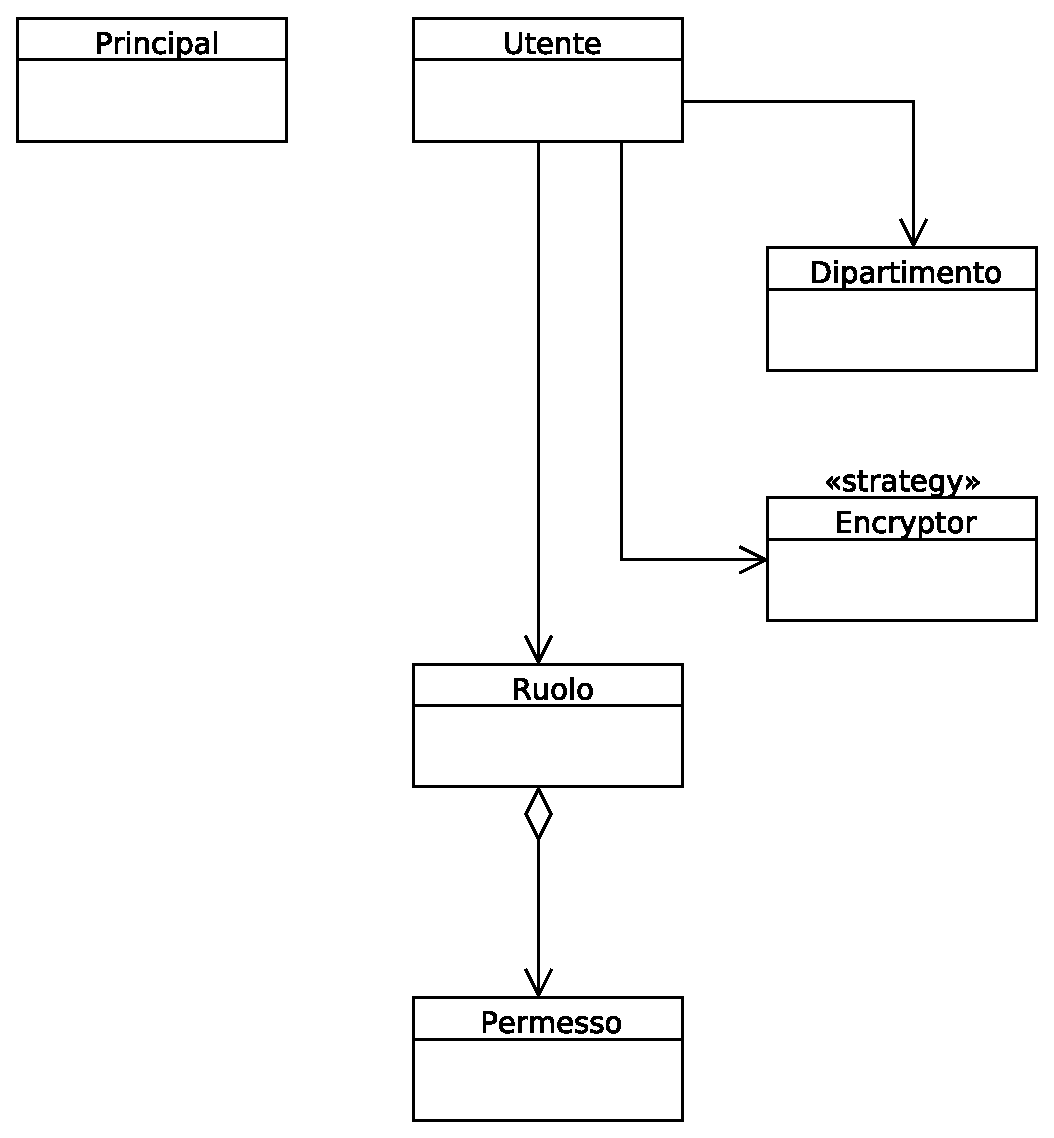
\includegraphics[width=0.4\textwidth]{user_model_final.eps}

\end{frame}

\subsection{Ruoli e Permessi}

\begin{frame}{Ruoli e Permessi}
\begin{itemize}
	
\item Operatore Amministrativo
	\begin{itemize}
	\item Gestisce le convenzioni del proprio dipartimento
	\end{itemize}

\vspace{0.8em}
\item Docente
	\begin{itemize}
	\item Visualizza le proprie convenzioni
	\item Allega documenti alle proprio convenzioni
	\end{itemize}

\vspace{0.8em}
\item Ospite
	\begin{itemize}
	\item Nessun permesso
	\end{itemize}

\vspace{0.8em}
\item Amministratore
	\begin{itemize}
	\item Gestisce gli utenti ed i loro permessi
	\item Non afferisce a nessun dipartimento
	\end{itemize}
\end{itemize}
\end{frame}

\section{Collaudo}
\subsection{Introduzione}
\begin{frame}{Collaudo}
\begin{itemize}
\item Verifica le funzionalità dell'applicazione
\vspace{0.8em}
\item Suddivisione in scenari con ragionevole copertura\newline
dei casi d'uso
\end{itemize}

\end{frame}

\begin{frame}{Scenari e Casi di test}

\begin{itemize}
\item Copertura dei casi d'uso
\end{itemize}

\begin{center}
\footnotesize
\begin{tabular}{| c| p{4.5cm} | p{4.5cm} |} 
    \hline
     & Descrizione & Casi di test esercitati \\
    \hline
    1 & Inserimento convenzione,\newline
    aggiunta ditta,
    aggiunta rata & UC \#OA1 base,
    UC \#OA10 alt3,\newline
    UC \#OA6 base\\
    \hline
    2 & Modifica rata contributo & UC \#OA2 base,
    UC \#OA3 base, \newline
    UC \#OA7 base  \\
    \hline
    3 & Modifica dati ditta & UC \#OA13 base,
    UC \#OA11 base \\
    \hline
    4 & Inserimento contributo con allegati & UC \#OA1 base\\
    \hline
    5 & Inserimento allegato convenzione & UC \#D1 base,
    UC \#D3 base\\
    \hline
    6 & Aggiunta utente & UC \#A1 base\\
    \hline
  \end{tabular} 
\end{center}

\end{frame}

\subsection{Risultati}

\begin{frame}{Risultati}
\begin{center}
\footnotesize
\begin{tabular}{|c|p{2.5cm}|p{3cm}|p{1.5cm}|c|}
    \hline
    Passo & Descrizione sequenza operazioni & Risultato
     atteso & Risultato\newline ottenuto & Ok\\
    \hline
    1 & L'Amministratore clicca sul pulsante\newline ``Aggiungi utente'' & Viene visualizzata una schermata contenente\newline i campi da inserire& Uguale 
      al\newline risultato\newline atteso& Sì\\
    \hline
    2 & L'Amministratore riempie i campi quindi clicca su ``Salva''& Si torna alla\newline pagina iniziale & Uguale al\newline risultato\newline atteso & Sì \\
    \hline
     3 & L'Amministratore clicca su ``Visualizza lista utenti''& Compare una lista contenente tutti gli utenti, fra i quali anche quello appena inserito & Uguale al\newline risultato\newline atteso & Sì \\
    \hline
\end{tabular}
\end{center}

\end{frame}

\section{Conclusioni}
\begin{frame}{Riassunto}
\begin{itemize}
\item Copertura del ciclo di sviluppo di un'applicazione
	\vspace{0.6em}
	\begin{itemize}
	\item requisiti acquisiti da un'audience informata
	\vspace{0.4em}
	\item applicazione progettata, sviluppata, collaudata e\newline
	pronta per andare in produzione (DINFO, DIEF, DICEA)
	\end{itemize}
\vspace{1em}
\item Ulteriori sviluppi abilitati
\vspace{0.6em}
\begin{itemize}
\item gestione dei contratti
\vspace{0.4em}
\item autorizzazioni ad incarichi retribuiti
\end{itemize}
\end{itemize}

\end{frame}
\begin{frame}{Requisiti}
\begin{itemize}
\item Gestione delle convenzioni e dei contributi
\vspace{0.8em}
	\begin{itemize}
	\item inserire convenzioni
	\item inserire rate per una convenzione
	\item visualizzare convenzioni inserite
	\item aggiornare i dati di una convenzione
	\item notificare le scadenze
	\end{itemize}
\end{itemize}
\end{frame}

\begin{frame}{Conclusioni}
\begin{columns}[T]
\begin{column}{.3\textwidth}
\begin{itemize}
\item Tecnologie
\vspace{0.8em}
	\begin{itemize}
	\item JPA
	\vspace{0.6em}
	\item CDI
	\vspace{0.6em}
	\item JSF
	\vspace{0.6em}
	\item Deltaspike
	\vspace{0.6em}
	\item LDAP
\end{itemize}
\end{itemize}
\end{column}

\begin{column}{.55\textwidth}

\centering
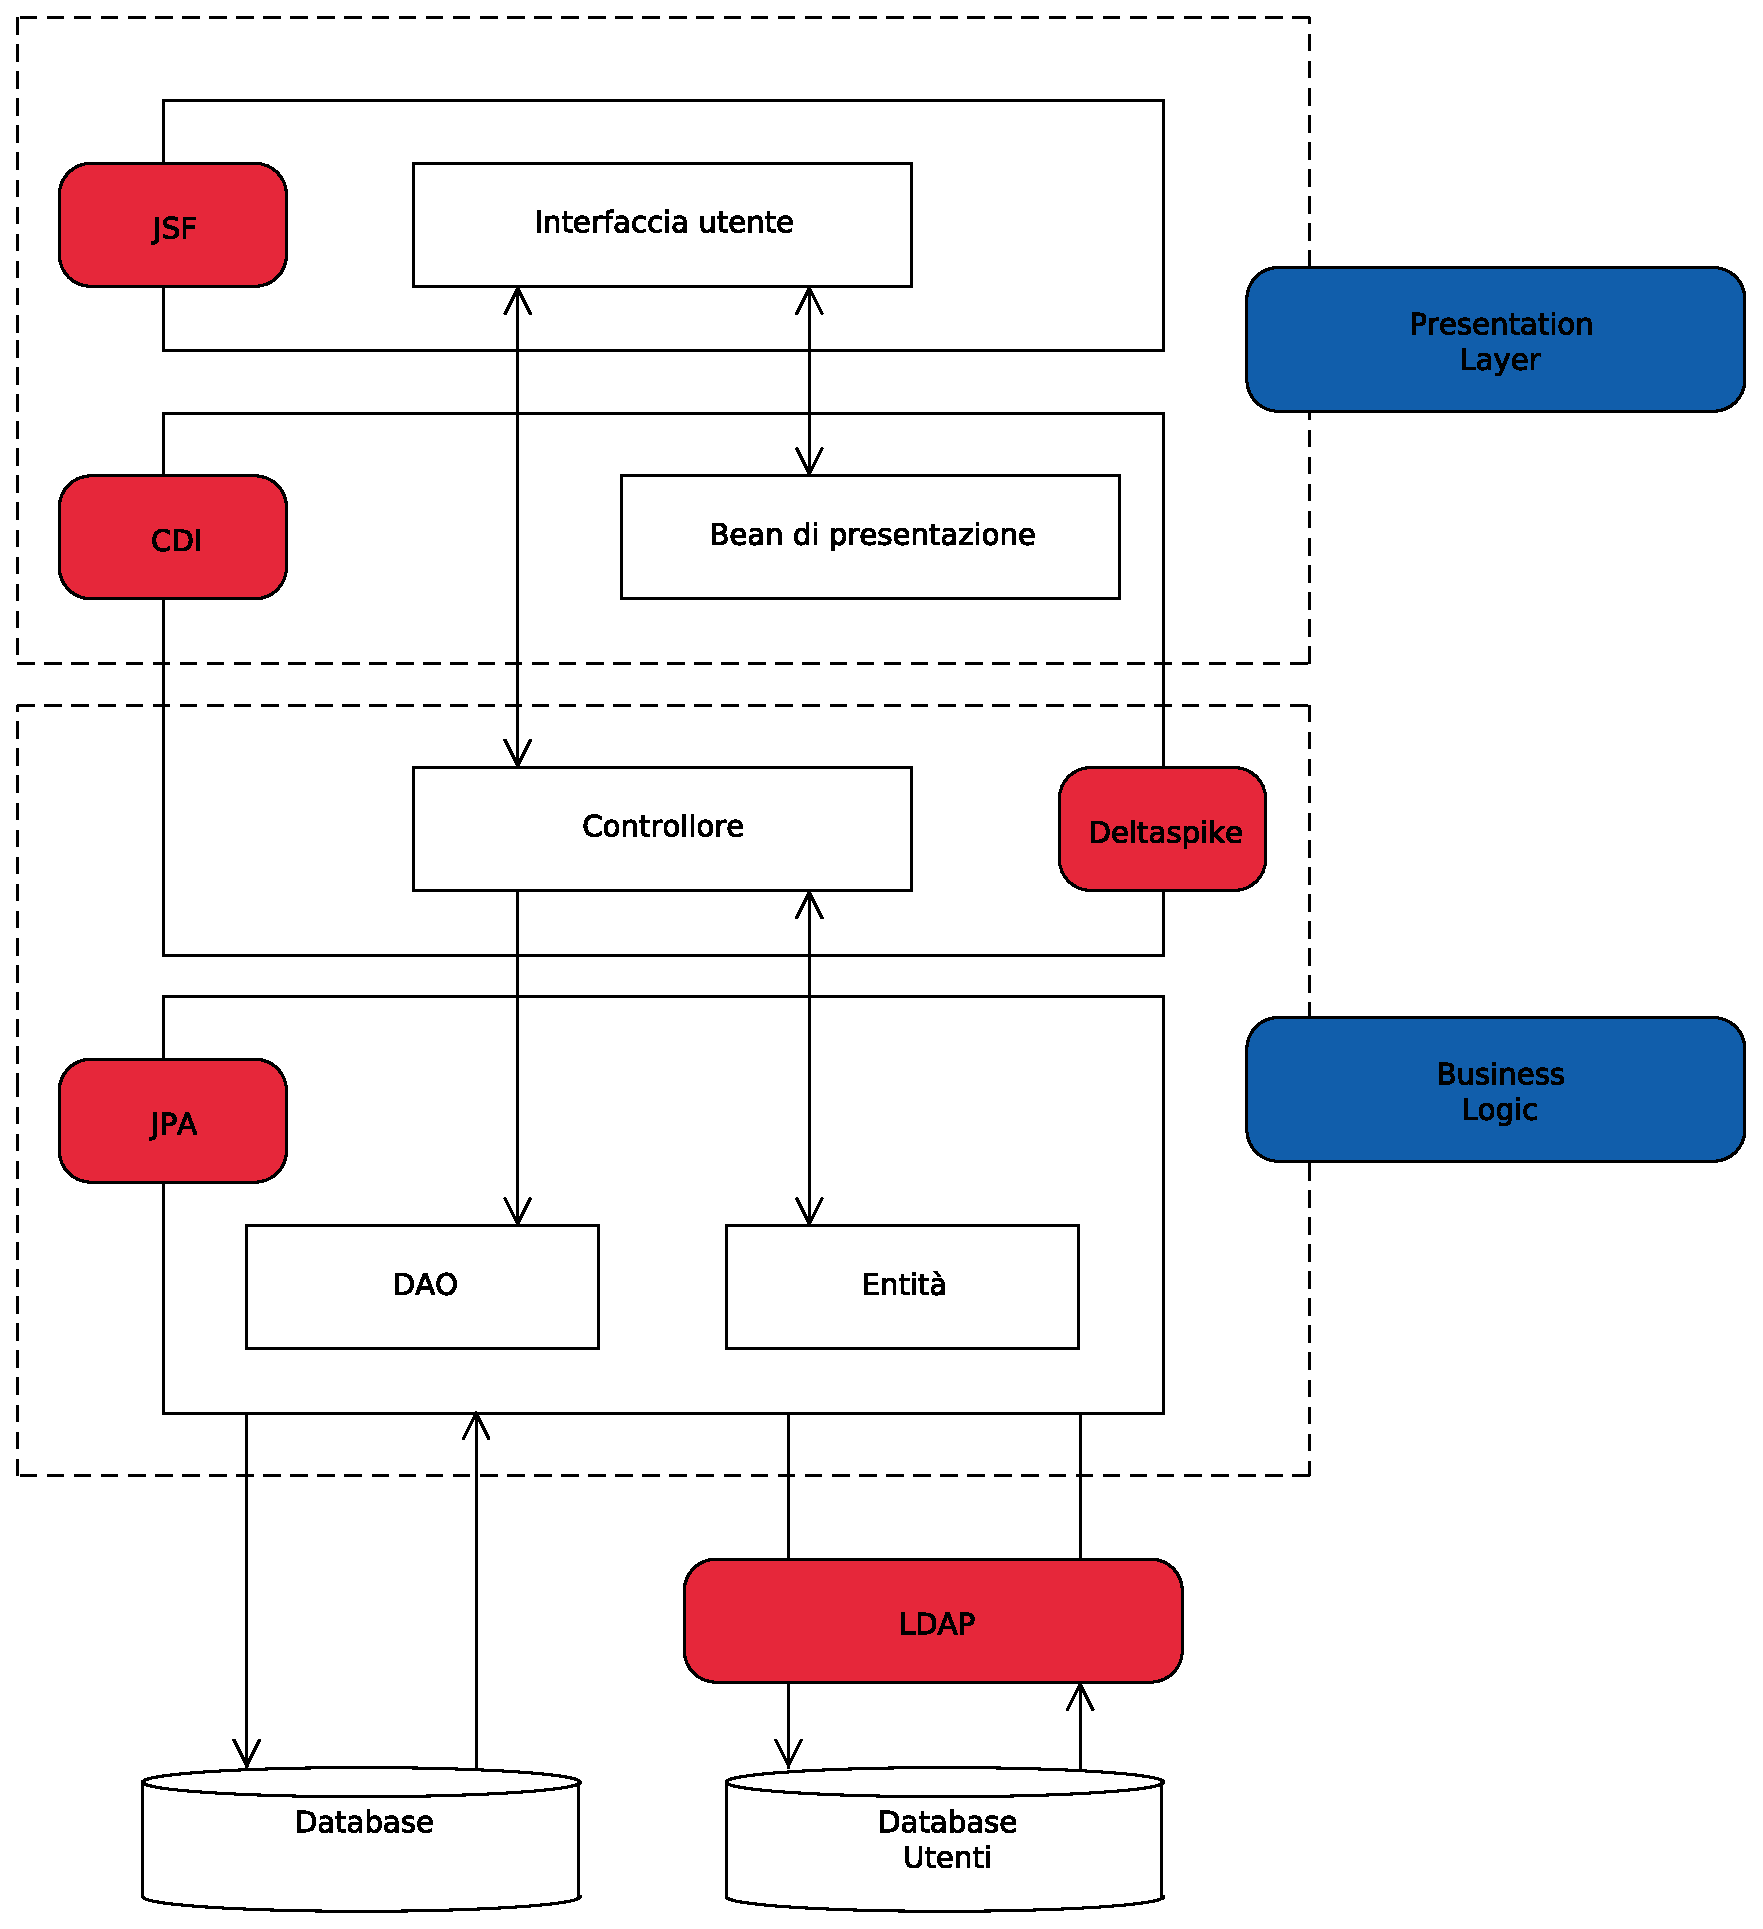
\includegraphics[width=1\textwidth]{tech_architecture_final.eps}

\end{column}
\end{columns}

\end{frame}